\chapter{Εισαγωγή}

\epigraph{\textquote{Η επιτυχημένη δημιουργία [γενικευμένης] Τεχνητής Νοημοσύνης θα είναι το μεγαλύτερο γεγονός στην ανθρώπινη ιστορία. Δυστυχώς, ίσως είναι και το τελευταίο εάν δε μάθουμε πώς να αποφεύγουμε τα ρίσκα.}{ --- \textup{\en{Stephen Hawking}}}}

\section{Επισκόπηση του Κόσμου της Τεχνητής Νοημοσύνης}

Είναι πλέον γεγονός, η Τεχνητή Νοημοσύνη (\en{Artificial Intelligence - AI}) εντοπίζεται σε πολλές εκφάνσεις της καθημερινότητας των περισσότερων ανθρώπων \cite{smith_.i._2021}.
Δεν αποτελεί απλά έναν ακόμα μοδάτο όρο που καταχράται στον χώρο της αγοραστικής (\en{marketing}). Εν αντιθέσει, διαδραματίζει καθοριστικό ρόλο στην εργασία μας, στη μετακίνησή μας 
και στην ψυχαγωγία μας. Για παράδειγμα, εντοπίζεται στις μηχανές αναζήτησης όπως η \en{Google}, στους ηλεκτρονικούς χάρτες πλοήγησης αλλά και στα συστήματα συστάσεων (\en{Recomender systems}) 
όπως αυτό του \en{YouTube}, του \en{Twitter} και του \en{Netflix} \cite{marr_10_nodate} που εξατομικεύουν το προβαλλόμενο περιεχόμενο στα ενδιαφέροντα του χρήστη. 
\par

Η επιρροή που έχει η Τεχνητή Νοημοσύνη είναι ακόμα πιο ευδιάκριτη αν τη μελετήσει κανείς υπό μια συλλογική σκοπιά. 
Για παράδειγμα, στον χώρο του επιχειρείν, η αξιοποίηση τεχνολογιών Τεχνητής Νοημοσύνης έχει αποδειχθεί ότι αυξάνει την επιχειρηματική αξία (\en{business value}) μέσα από τη βελτίωση της επίδοσης τόσο στο οικονομικό (\en{financial}), αγοραστικό (\en{marketing}) και διοικητικό (\en{administrative}) επίπεδο όσο και στο επίπεδο επιχειρηματικών διαδικασιών (\en{business process}) \cite{wamba2020influence}. Χαρακτηριστικό παράδειγμα αποτελεί η χρήση των συστημάτων συστάσεων αφού με το να φιλτράρουν το περιεχόμενο και να παρουσιάζουν στον χρήστη μόνο αυτό που του είναι οικείο και θεμιτό, αυξάνουν τον βαθμό ενασχόλησής του με κίνδυνο την παγίδευσή του σε μια \textquote{φούσκα προκατειλημμένου φιλτραρίσματος} (\en{\textquote{biased filter bubble}}) \cite{fernandez2021analysing}. Άλλωστε, όπως δηλώνει η ομάδα ανάπτυξης του εν λόγω συστήματος για λογαριασμό της συνδρομητικής υπηρεσίας \en{streaming}, \en{Netflix}, \textquote{Πιστεύουμε ότι αθροιστικά, η επίδραση της εξατομίκευσης και των συστάσεων μας εξοικονομεί ένα δισεκατομμύριο δολάρια τον χρόνο} \cite{gomez2015netflix}.
\par

Στον εργασιακό χώρο, πολλές δουλειές που περιλαμβάνουν επαναλαμβανόμενες, προβλέψιμες εργασίες κυρίως στον τομέα της βιομηχανίας και της γεωργίας αντικαθίστανται από αυτοματισμούς Τεχνητής Νοημοσύνης (\en{AI automations}) εκτοπίζοντας έτσι τον άνθρωπο. 
Η μείωση των διαθέσιμων θέσεων εργασίας στους τομείς αυτούς δοκιμάζει τα όρια του κοινωνικού οικοδομήματος: τα \textquote{εκτοπισμένα} άτομα καλούνται να αποκτήσουν νέες δεξιότητες προκειμένου να βρουν απασχόληση στις πιο δημιουργικές (και συνάμα λιγότερο τυποποιήσιμες) θέσεις του εξελισσόμενου τομέα των υπηρεσιών \cite{makridakis2017forthcoming}. Βέβαια, η μείωση των θέσεων εργασίας επαναλαμβανόμενης φύσης είναι μόνο η μια πλευρά του νομίσματος. Σύμφωνα με αναλύσεις, μέχρι την επόμενη δεκαετία οι εφαρμογές της Τεχνητής Νοημοσύνης εν δυνάμει θα αυξήσουν το παγκόσμιο Ακαθάριστο Εθνικό Προϊόν (\en{Gross Domestic Product - GDP}) κατά 26\% (δεκαπέντε τρισεκατομμύρια δολάρια) \cite{hawksworth2018will}. Αυτό, με τη σειρά του, θα οδηγήσει στη δημιουργία πολλών νέων θέσεων εργασίας έτσι ώστε να μην παρατηρηθεί αύξηση στους δείκτες ανεργίας \cite{hawksworth2018will,world2020future}.
\par

Τέλος, δε θα μπορούσαμε να παραλείψουμε την επιρροή που έχει η Τεχνητή Νοημοσύνη στον χώρο της υγείας. Οι εφαρμογές είναι ατελείωτες: από συστήματα για πρόωρη διάγνωση ασθενειών μέχρι ρομποτικά συστήματα υποβοήθησης χειρουργείου \cite{tai2020impact}. Αξιοσημείωτη είναι επίσης η επιτυχημένη εφαρμογή της για την πρόβλεψη της τρισδιάστατης δομής των πρωτεϊνών \cite{senior2020improved} - ένα θέμα με σημαντικές προεκτάσεις που απασχολούσε την επιστημονική κοινότητα για 50 χρόνια. Παρόλα αυτά, μαζί με την προσπάθεια για αξιοποίηση των νέων τεχνολογιών στην κλινική πράξη προκύπτουν νέες προκλήσεις. Μια πρώτη δυσκολία είναι η ανάπτυξη συστημάτων Τεχνητής Νοημοσύνης που απαιτούν μεγάλο όγκο δεδομένων σε χώρους προβλημάτων όπου αυτά σπανίζουν (όπως για παράδειγμα, στην περίπτωση μιας ασυνήθιστης ασθένειας όπου ο αριθμός των ιατρικών υποθέσεων είναι ελάχιστος). Αυτή η δυσκολία εντείνεται αφενός λόγω της έλλειψης ασφαλών υποδομών για τη συλλογή ιατρικών δεδομένων \cite{panch2019inconvenient} και αφετέρου λόγω της απόρρητης φύσης αυτών, κάτι που δυσχεραίνει τον ελεύθερο διαμοιρασμό τους. Μια τελευταία δυσκολία αποτελεί το γεγονός ότι πολλά συστήματα Τεχνητής Νοημοσύνης που έχουν αναπτυχθεί σε περιβάλλον εργαστηρίου (\en{Lab setting}) δεν παρέχουν αρκετά κίνητρα για μεταστροφή της καθιερωμένης κλινικής πράξης \cite{panch2019inconvenient}. Για να επιτευχθεί κάτι τέτοιο, μεταξύ άλλων θα πρέπει τα συστήματα να αποδίδουν αποδεδειγμένα τόσο καλά όσο και το καταρτισμένο προσωπικό στο συγκεκριμένο πεδίο εφαρμογής τους και να παρέχουν πληροφορίες που θα τα καθιστούν περισσότερο έμπιστα π.χ. αιτιολογώντας την απόφασή τους (\en{explainability}),  παρέχοντας μια μετρική αβεβαιότητας (\en{uncertainty}) ή δίνοντας τη δυνατότητα αλληλεπίδρασης \cite{rajkomar2019machine}.
\par

Αντιλαμβανόμενοι το εύρος των εφαρμογών της Τεχνητής Νοημοσύνης, 
η εκτίμηση από την \en{International Data Corporation - IDC} πως οι Ευρωπαϊκές δαπάνες σε τέτοιες εφαρμογές θα έχουν σχεδόν τριπλασιαστεί μέσα στα επόμενα τρία χρόνια δε θα πρέπει να μας εκπλήσσει. Ωστόσο, με τη μεγάλη ισχύ έρχεται και μεγάλη ευθύνη. Είναι αλήθεια, η Τεχνητή Νοημοσύνη είναι ήδη εδώ και θα συνεχίζει να επιδρά όλο και εντονότερα στην καθημερινότητα μας και στην κοινωνία. Βέβαια, η σημερινή Τεχνητή Νοημοσύνη είναι εντελώς διαφορετική από αυτό που φαντάζονταν η κοινή γνώμη τις προηγούμενες δεκαετίες (σαφώς επηρεασμένη από ταινίες επιστημονικής φαντασίας όπως το \en{Terminator}). Θα λέγαμε, αντίθετα, πως εμφανίζεται περισσότερο με μια περιορισμένη μορφή στην εκάστοτε συγκεκριμένη εφαρμογή (\en{narrow AI}). Έτσι, ένα \textquote{εφυές} σύστημα για μια εργασία δεν μπορεί να \textquote{γενικεύσει} και να εφαρμοστεί σε άλλο χώρο προβλημάτων. Ούτε λόγος δε για αισθήματα και υπαρξιακή συνείδηση· αυτά (ακόμα) ανήκουν στην επιστημονική φαντασία. 
Αυτό όμως δε σημαίνει ότι η επιπόλαιη χρήση της Τεχνητής Νοημοσύνης δεν ελοχεύει κινδύνους. Σύμφωνα με το περιοδικό \en{Spectrum} της \en{IEEE} \cite{bajema_ais_2022} προτού επιτευχθεί Τεχνητή Νοημοσύνη επιπέδου ανθρώπου (\en{human-like Artificial Inteligence}) - αυτή στην οποία αναφέρεται ο \en{Stephen Hawking} - υπάρχουν ήδη πολλά σενάρια όπου εφαρμογές της μπορούν να αποβούν μοιραίες. Ενδεικτικά, ένα από αυτά είναι τα \en{deepfakes} - ψεύτικα πολυμέσα βίντεο και εικόνας κατασκευασμένα από εφαρμογές Τεχνητής Νοημοσύνης - έχουν υπονομεύσει την εμπιστοσύνη στα συστήματα πληροφόρησης. Επιπρόσθετα, ένα ακόμα καταστροφικό σενάριο σχετίζεται με την ιδιωτικότητα (\en{privacy}) και την ελεύθερη βούληση (\en{free will}). Με την παραχώρηση ευαίσθητων δεδομένων σε επιχειρήσεις και κυβερνήσεις τους παρέχουμε τη δυνατότητα να μας εποπτεύουν ακόμα και να μας χειραγωγούν. Ένα τελευταίο σενάριο για το οποίο διαδραματίζουν άμεσο ρόλο τα κοινωνικά δίκτυα είναι αυτό του μειωμένου διαστήματος προσοχής (\en{short attention span}) ως απόρροια της εκμετάλλευσης του μηχανισμού επιβράβευσης του εγκεφάλου ώστε οι χρήστες να εθίζονται σε αυτά. Το περιοδικό καλεί τον αναγνώστη να αναλογιστεί τις συνέπειες της συνεχόμενης βελτίωσης των μηχανισμών που μας καθηλώνουν από τη νέα τεχνολογία. Συμπερασματικά, η Τεχνητή Νοημοσύνη αν και δεν προσομοιάζει την ανθρώπινη νοημοσύνη δεν παύει να αποτελεί μια πολύ ισχυρή τεχνολογία που μπορεί να αποβεί είτε σωτήρια είτε μοιραία ανάλογα με τον τρόπο αξιοποίησής της.
\par

Είναι λοιπόν απαραίτητη η εξασφάλιση της συνετής χρήσης αυτών των τεχνολογιών μέσω μιας σειράς κανονισμών. Στην Ευρωπαϊκή Ένωση, μια σειρά από διατάξεις επιχειρούν να θέσουν ένα νομοθετικό πλαίσιο ώστε να ωθήσουν στην αξιοποίηση της Τεχνητής Νοημοσύνης διασφαλίζοντας παράλληλα την ασφάλεια των θεμελιωδών δικαιωμάτων \cite{europeancomissionai2021}. Άλλωστε, σύμφωνα με την \en{von der Lein} \cite{VonderLeyen2019}, \textquote{Η Τεχνητή Νοημοσύνη πρέπει να εξυπηρετεί τους ανθρώπους και  συνεπώς, πρέπει πάντα να συμμορφώνεται με τα δικαιώματά τους. Αυτός είναι ο λόγος που ένα άτομο πρέπει πάντα να έχει τον έλεγχο στην περίπτωση κρίσιμων αποφάσεων[…] Εφαρμογές της Τεχνητής Νοημοσύνης που μπορεί να παρέμβουν στα ανθρώπινα δικαιώματα θα πρέπει να ελέγχονται και να πιστοποιούνται πριν φτάσουν στην Ευρωπαϊκή αγορά. } Αν και οι αυστηροί διακανονισμοί καθυστερούν τη μετάβαση εφαρμογών Τεχνητής Νοημοσύνης από το εργαστήριο στην αγορά, εξασφαλίζουν την ασφάλειά τους συμβάλλοντας στην αξιοπιστία τους.
\par

Με την παραπάνω σύντομη εισαγωγή καλύψαμε εμπεριστατωμένα πολλά από τα μη τεχνικά θέματα που σχετίζονται με την Τεχνητή Νοημοσύνη (\en{Artificial Inteligence}).
Αναλυτικότερα, αρχίσαμε από παραδείγματα εντοπισμού της στην καθημερινή ζωή σε ατομικό και σε συλλογικό επίπεδο με τα οποία αντιληφθήκαμε τη σημασία της. Συνεχίσαμε με τους κινδύνους που ελοχεύει η απερίσκεπτη εφαρμογή της σε συγκεκριμένες εργασίες επισημαίνοντας ταυτόχρονα ότι η τεχνητή νοημοσύνη απέχει από την ανθρώπινη. Κλείσαμε, με μερικές από τις προσπάθειες που γίνονται σε Ευρωπαϊκό επίπεδο για την αποφυγή αυτών των κινδύνων.
Πολλά από τα προαναφερθέντα στοιχεία πιθανότατα να είναι ήδη γνωστά σε έναν έμπειρο αναγνώστη. Εντούτοις, εξυπηρετούν σε μια ομαλή εισαγωγή για τον αρχάριο και σε μια υπενθύμιση για τον έμπειρο αναγνώστη του κόσμου της Τεχνητής Νοημοσύνης.
Στην επόμενη υπο-ενότητα αυτού του κεφαλαίου θα παρουσιάσουμε μια ιστορική αναδρομή της τεχνητής νοημοσύνης. Έτσι, ο αναγνώστης θα κατανοήσει σε βάθος την έννοια γύρω από την οποία εκτυλίσσεται η παρούσα διπλωματική προτού εισαχθεί στο συγκεκριμένο τεχνικό της θέμα. Έπειτα, περιγράφεται το κίνητρο που με ωθούσε καθ'όλη τη διάρκεια συγγραφής του έργου. Τέλος, αναφερόμαστε στην τεχνική συνεισφορά της παρούσας εργασίας και στην οργάνωση του τόμου.



\section[Ιστορική Αναδρομή Τεχνιτής Νοημοσύνης]{Ιστορική Αναδρομή Τεχνητής Νοημοσύνης}

Οι εφευρέτες οραματίζονται εδώ και χιλιετίες τη δημιουργία μηχανών που σκέφτονται. Ήδη, γύρω στο 700 π.Χ. αναφέρεται από τον Ησίοδο ο Τάλος: ο μυθικός χάλκινος γίγαντας φτιαγμένος από τον Ήφαιστο με αποστολή να προστατεύσει το νησί της Κρήτης από τους επιδρομείς \cite{mayor2020gods}. Παρόμοια παραδείγματα αποτελούν αυτά της Πανδώρας και της Γαλάτειας. Η μακρόβια επιθυμία για απομίμηση της νοημοσύνης μαρτυρά την αξία που της δίνει ο άνθρωπος. Γεγονός απόλυτα δικαιολογημένο αφού η νοημοσύνη - η νοητική ικανότητα που μας επιτρέπει να σκεπτόμαστε λογικά, να επιλύουμε προβλήματα και να μαθαίνουμε - έχει συμβάλει σημαντικά στην επιβίωση του είδους από τον διαειδικό ανταγωνισμό (\en{interspecific competition})\footnote{Για την ακρίβεια, ενώ σύμφωνα με τη Δαρβινική θεώρηση η αφηρημένη νοημοσύνη μπορεί να προκύψει άμεσα από τη θεωρία της εξέλιξης των ειδών, νεότερες έρευνες το διαψεύδουν αφού το χαρακτηριστικό της αφηρημένης σκέψης ήταν αχρείαστο στην πραγματιστική παλαιολιθική εποχή. Στην προσπάθειά τους να ερμηνεύσουν την εμφάνιση νοημοσύνης στους ανθρώπους ορίζουν τον όρο \textquote{διανοητική βιοθέση} (\en{cognitive niche}) για να περιγράψουν όλα τα ζωολογικά ασυνήθιστα χαρακτηριστικά (\en{zoologically unusual traits}) που εμφανίζει ο άνθρωπος με τα κυριότερα να είναι η κοινωνικότητα και η λογική αιτίου - αποτελέσματος (\en{cause-and-effect reasoning}) \cite{pinker2010cognitiveniche,tooby1987reconstruction}. Υποστηρίζουν λοιπόν, ότι η εμφάνιση της διανοητικής βιοθέσης αποτέλεσε τον καταλύτη για την εξέλιξη της ανθρώπινης νοημοσύνης \cite{avise2010light}}. Σε τελική ανάλυση, ο όρος \en{homo sapiens} - άνθρωπος ο σοφός - οφείλεται στη σημασία που έχει η νοημοσύνη στη ζωή μας.
\par

Το πρώτο ευρέως αναγνωρισμένο έργο προς την επίτευξη Τεχνητής Νοημοσύνης είναι αυτό της μαθηματικής μοντελοποίησης της λειτουργίας ενός νευρώνα από τους \en{Warren McCulloch} και \en{Walter Pitts} (1943) \cite{mcculloch1943logical}. Αναλυτικότερα, βασιζόμενοι στην υπόθεση ότι η κατάσταση λειτουργίας ενός νευρώνα είναι δυαδική (\en{\textquote{all-or-none}}) αναπαρέστησαν κάθε νευρώνα ενός δικτύου ως μια πρόταση (\en{proposition}) της προτασιακής λογικής (\en{propositional logic}). Όπως περιγράφουν, η διέγερση (\en{excitation}) του μοντέλου ενός νευρώνα είναι ταυτόσημη με το να είναι η πρόταση του νευρώνα θετική, κάτι που εξαρτάται από την κατάσταση των γειτονικών νευρώνων. Όσο περισσότεροι, διεγερτικά διασυνδεδεμένοι (\en{excitatory connected}) προσυναπτικοί νευρώνες (\en{presynaptic neurons}) είναι ενεργοποιημένοι τόσο πιο πιθανή είναι η ενεργοποίηση του μετασυναπτικού νευρώνα (\en{postsynaptic neuron}). Μεταξύ άλλων, απέδειξαν ότι κάθε συνάρτηση που μπορεί να υπολογιστεί από μια μηχανή \en{Turing} μπορεί να υπολογιστεί και από ένα δίκτυο από διασυνδεδεμένους τεχνητούς νευρώνες ύστερα από την κατάλληλη παραμετροποίησή του. Το έργο των \en{Warren McCulloch} και \en{Walter Pitts} ήταν πρωτοπόρο για την εποχή του αφού έθεσε τις βάσεις όχι μόνο για την σημερινή Τεχνητή Νοημοσύνη αλλά και για την Υπολογιστική Νευρωεπιστήμη (\en{Computational Neuroscience}). Ωστόσο, οι συγγραφείς δεν παρουσίασαν κανέναν αλγόριθμο για την αλλαγή της τοπολογίας και των παραμέτρων του τεχνητού νευρωνικού δικτύου αν και φαίνεται πως αναγνώριζαν τη σημασία του για τη μάθηση. 
\par

Στο βιβλίο του \cite{hebb1949organization} ο \en{D. Hebb} το 1949 επιδίωξε να ενώσει τις αποκλίνουσες θεωρίες της ψυχολογίας και της νευροεπιστήμης θέτοντας κοινές βάσεις για την ερμηνεία της ανθρώπινης συμπεριφοράς. Προηγούμενες θεωρίες απέφευγαν να δώσουν εξήγηση στις διεργασίες του εγκεφάλου ως μεσάζοντα μεταξύ του αισθητηριακού ερεθίσματος (\en{sensory stimuli}) και της πιθανής, καθυστερημένης απόκρισης. Αντίθετα, κατέφευγαν στη φιλοσοφία για την ανάλυση των χαρακτηριστικών της ανθρώπινης συμπεριφοράς όπως η προσοχή (\en{attention}), το ενδιαφέρον (\en{interest}) και η \textquote{προσδοκία} (\en{expectancy}). Ο \en{Hebb} όμως, εργάστηκε στο να αποδείξει ότι η ανθρώπινη συμπεριφορά μπορεί να γίνει κατανοητή υπό το πρίσμα της φυσιολογίας (\en{"[expectancy] can be a physiologically intelligible process"}). Φαινομενικά, ενώ το έργο του απασχολεί μόνο την επιστήμη της Νευροφυσιολογίας (\en{Neurophysiology}) συνεισέφερε σημαντικά στο κίνημα του διασυνδετισμού (\en{Connectionism}) - το κίνημα μελέτης των διανοητικών διεργασιών με τη χρήση τεχνητών νευρωνικών δικτύων. Για παράδειγμα, η θεώρηση της διαδικασίας μάθησης ως της επαναλαμβανόμενης, ταυτόχρονης πυροδότησης γειτονικών νευρώνων με αποτέλεσμα [την ενδυνάμωση των δεσμών και] τη διαμόρφωση νευρικών συστάδων (\en{cell assemblies}) είναι η λογική πίσω από πολλούς αλγορίθμους μάθησης τεχνητών νευρωνικών δικτύων. Επίσης, ένα στοιχείο που θα μας φανεί χρήσιμο στη συνέχεια είναι η παρατήρησή του ότι η κίνηση των ματιών δεν είναι τυχαία αλλά σχετίζεται με τη διαδικασία αντίληψής των θωρούμενων αντικειμένων. Τα παραπάνω δύο έργα έθεσαν το απαραίτητο θεωρητικό υπόβαθρο εμπνέοντας τους ερευνητές στην πειραματική υλοποίηση της Τεχνητής Νοημοσύνης.
\par

Αρκετές ήταν οι απόπειρες δημιουργίας Τεχνητής Νοημοσύνης. Ο πρώτος υπολογιστής τεχνητών νευρωνικών δικτύων ονομάζονταν \en{SNARC} (\en{Stochastic Neural Analog Reinforcement Calculator}) και κατασκευάστηκε από τους \en{Marvin Minsky} και \en{Dean Edmonds} το 1950 \cite{akst_2019}. Χρησιμοποιώντας 3000 λυχνίες κενού και έναν μηχανισμό αυτόματου πιλότου εξομοίωσαν τη λειτουργία 40 διασυνδεδεμένων νευρώνων. Χρησιμοποιώντας έναν απλό μηχανισμό επιβράβευσης τα \textquote{βάρη} του δικτύου - υπο τη μορφή ποτενσιόμετρων - προσαρμόζονταν  στο πρόβλημα του λαβυρίνθου στο οποίο δοκιμάστηκε. Ακόμα ένα παράδειγμα τεχνητής νοημοσύνης μπορεί να θεωρηθεί το πρόγραμμα του \en{Christopher Strachey} στον υπολογιστή \en{Manchester Mark 1} \cite{lee1995computer} που αργότερα θεωρήθηκε το πρώτο βιντεοπαιχνίδι. Ήταν ένα παιχνίδι ντάμας που πιθανώς χρησιμοποιούσε κάποιον μη πλήρη (\en{incomplete}) αλγόριθμο αναζήτησης στον χώρο των επιτρεπτών ακολουθιών κινήσεων (\en{action sequences}). Παρόλα αυτά, η δυνατότητά του να ανταγωνίζεται αποτελεσματικά τον άνθρωπο οδήγησε στη θεώρησή του ως Τεχνητή Νοημοσύνη. Άλλωστε, η σύγχυση για το θέμα ήταν ακόμα μεγαλύτερη την εποχή εκείνη. 
\par

Ο αρχικός ενθουσιασμός για το επιστημονικό πεδίο τράβηξε τα βλέμματα πολλών επιφανών ερευνητών της εποχής. Ο πατέρας της Επιστήμης των Υπολογιστών (\en{Computer Science}) και της Τεχνητής Νοημοσύνης, \en{Alan Turing}, στην προσπάθειά του να διασαφηνίσει το ερώτημα του \textquote{αν οι μηχανές σκέφτονται} επινόησε το επονομαζόμενο \en{Turing Test}. Σύμφωνα με τη δημοσίευσή του \cite{TURING/10.1093/mind/LIX.236.433} το 1950, πρόκειται για μια δοκιμασία που εμπλέκει έναν \textquote{ανακριτή} ο οποίος διατυπώνει γραπτές ερωτήσεις σε δύο \textquote{μάρτυρες}: έναν άνθρωπο και μια μηχανή. Η δοκιμασία θεωρείται επιτυχής όταν ο ανακριτής - χωρίς να έχει οπτική επαφή με τους \textquote{μάρτυρες} - δεν μπορεί να ξεχωρίσει τον άνθρωπο από τη μηχανή. Στην ίδια δημοσίευση τόνισε τη σημασία της μάθησης για την ανάπτυξη της Τεχνητής Νοημοσύνης. Υποστήριζε ότι αντί να επιχειρείται η εξονυχιστική συγγραφή ενός προγράμματος που θα μοιάζει με τη σκέψη ενός ώριμου ενήλικα (με αμέτρητες προγραμματισμένες εντολές) είναι προτιμότερη και ταχύτερη η προσομοίωση της νοημοσύνης ενός παιδιού που μέσα από μηχανισμούς εκπαίδευσης, έμμεσα, αποκτά ώριμη σκέψη. Επίσης, εναπόθεσε τους σπόρους για τους γενετικούς αλγορίθμους, ενώ σε επόμενη δημοσίευσή του \cite{turing1948intelligent} μελέτησε τους τρόπους με τους οποίους μια μηχανή με νοημοσύνη θα μπορούσε να λειτουργεί. Ένα ακόμα δημοφιλές όνομα, ο \en{John von Neumann} συνεισέφερε στον χώρο αναπτύσσοντας τα \textquote{τεχνητά αυτόματα} (\en{artificial automata}) \cite{muehlenbein2014artificial} ενώ η συμβολή του πιθανώς θα ήταν ακόμα μεγαλύτερη αν προλάβαινε να ολοκληρώσει το βιβλίο του \textquote{Ο Υπολογιστής και το Μυαλό} (\en{The Computer and the Brain}). Μια τελευταία απόδειξη της προσοχής που έλαβε η Τεχνητή Νοημοσύνη διαφαίνεται στα δέκα μέλη σχετικού σεμιναρίου (\en{workshop}) που έλαβε χώρα το καλοκαίρι του 1955 στο \en{Dartmouth College}\cite{russell2020artificial}. Ίσως το ποιο σημαντικό πόρισμα αυτής της συνάθροισης ήταν η ανάπτυξη του \en{Logic Theorist} από τους \en{Allen Newell} και \en{Herbert Simon}, ενός συστήματος για την απόδειξη θεωρημάτων στα μαθηματικά.
\par

Η δεκαετία που ακολούθησε χαρακτηρίζεται από έντονη αισιοδοξία για τις δυνατότητες της Τεχνητής Νοημοσύνης: γενναιόδωρες επενδύσεις σε ερευνητικά προγράμματα ενθάρρυναν τη δημιουργία ποικίλων προγραμμάτων που υποδείκνυαν κάποια μορφή νοημοσύνης. Πιο συγκεκριμένα, αν εξαιρέσουμε την εξέχουσα δουλειά του \en{Arthur Samuel} όπου ανέπτυξε ένα παιχνίδι ντάμας χρησιμοποιώντας ενισχυτική μάθηση (\en{Reinforcement Learning}), οι περισσότερες προσπάθειες εστίασαν στον χώρο της μίμησης της ανθρώπινης συλλογιστικής (\en{reasoning}). Η ιδέα είναι ότι με μια τυπική γλώσσα (\en{formal language}) για την αναπαράσταση της γνώσης (\en{knowledge representation}) στον υπολογιστή μαζί με την εφαρμογή απλών κανόνων λογικής συμπερασματολογίας (\en{logical inference}) σε αυτή καθιστούν δυνατή την εξαγωγή πορισμάτων. Καθοριστικό ρόλο σε αυτή τη \textquote{σχολή} είχε η - αναχρονιστική - υπόθεση ότι η νοημοσύνη είναι άρρηκτα συνδεδεμένη με τη δυνατότητα χειρισμού συμβόλων οργανωμένων σε δομές δεδομένων (\en{physical symbol system hypothesis}). 
\par

Σε αυτήν την κατεύθυνση, δηλαδή της συμβολικής Τεχνητής Νοημοσύνης (\en{Symbolic Artificial Inteligence}), εργάστηκαν αρκετοί επιστήμονες της εποχής. Για παράδειγμα, οι δύο ερευνητές πίσω από το \en{Logic Theorist} επινόησαν το \en{General Problem Solver}. Πρόκειται ουσιαστικά για έναν αλγόριθμο ο οποίος δέχεται σαν είσοδο μια τυποποιημένη περιγραφή του προβλήματος και το επιλύει ακολουθώντας μια στρατηγική ευρετικής αναζήτησης (\en{heuristic search}) της λύσης \cite{russell2020artificial}. Στο ίδιο μήκος κύματος εργάστηκε και ο \en{John McCarthy}. Εκτός από το ότι ανέπτυξε τη γλώσσα προγραμματισμού \en{Lisp}, ειδικά φτιαγμένη για εφαρμογές Τεχνητής Νοημοσύνης, εξέλιξε το πεδίο με το δημοσίευμά του \textquote{\en{Programs with Common Sense}} (1958) στο οποίο περιέγραφε το \en{Advice Taker}. Αυτό ήταν ένα πρόγραμμα για την επίλυση προβλημάτων μέσω της εφαρμογής \textquote{κοινής λογικής} σε προτάσεις διατυπωμένες σε τυπική γλώσσα. Για παράδειγμα, δοθέντος μιας σειράς υποθέσεων σχετικά με το περιβάλλον του προβλήματος διατυπωμένων σε τυπική γλώσσα (π.χ. \textquote{Εγώ είμαι στο γραφείο.}, \textquote{Θέλω να πάω αεροδρόμιο.} κτλ.) ο αλγόριθμος εξήγαγε ένα πλάνο με τα βήματα που πρέπει να ακολουθηθούν για τη μετάβαση στο αεροδρόμιο \cite{McCarthy1960ProgramsWC}. Το έργο του συνέχισε ο \en{J. A. Robinson} όπου και επινόησε μια πλήρη μέθοδο επίλυσης (\en{complete resolution method}) για προβλήματα εκφρασμένα σε λογική πρώτης τάξης. Οι εφαρμογές του ήταν πολλές: από συστήματα μαθηματικού λογισμού (\en{James Slagle's SAINT program} \cite{Slagle/10.1145/321186.321193} και \en{Daniel Bobrow's STUDENT program}) μέχρι εφαρμογές ερωταπαντήσεων (\en{Cordell Green's question-answering and planning systems}) και ρομποτικής (\en{Shakey Robotics Project}). Τέλος, πολλές εφαρμογές της Συμβολικής Τεχνητής Νοημοσύνης αναπτύχθηκαν για το \textquote{παιχνίδι} \en{blocks world}: ένα περιβάλλον αποτελούμενο από τουβλάκια που αποσκοπούσε στον πειραματισμό συστημάτων αναπαράστασης γνώσης και συλλογιστικής \cite{slaney2001blocks}.
\par

Την ίδια εποχή, ειδικά για τον χώρο των νευρωνικών δικτύων υπήρξε σημαντική πρόοδος με τα έργα \en{Perceptron} και \en{ADALINE}. Το πρώτο συγγράφηκε από τον \en{F. Rosenblatt} το 1958 και αποτέλεσε το πρώτο μοντέλο νευρωνικού δικτύου με δυνατότητα επιβλεπόμενης μάθησης \en{supervised learning}. Πιο συγκεκριμένα, το \en{Perceptron} είναι ένας ταξινομητής γραμμικά διαχωρίσιμων προτύπων με ένα μεμονωμένο τεχνητό νευρώνα του οποίου οι ελεύθεροι παράμετροι - τα προσυναπτικά βάρη (\en{presynaptic weights}) και η πόλωση (\en{bias}) - προσαρμόζονται στα δεδομένα εισόδου σύμφωνα με έναν αλγόριθμο μάθησης (\en{perceptron rule}) \cite{haykin2009neural}. Σε μια εκτενή παρουσίαση του έργου \cite{rosenblatt1958perceptron}, ο \en{Rosenblatt} βασίστηκε στη θεωρία του \en{D. Hebb} και την επέκτεινε προτείνοντας ένα μοντέλο (το \en{Perceptron}) με το οποίο η συμπεριφορά (καμπύλη εκμάθησης) μπορεί να προβλεφθεί από τη νευροφυσιολογία του συστήματος (τα συναπτικά βάρη). Παρόμοιο ήταν και το έργο \en{ADALINE} (\en{Adaptive Linear Neuron}) του \en{B. Widrow} στο οποίο περιγράφεται και πάλι ένας αλγόριθμος μάθησης για την προσαρμογή των βαρών. Αυτή τη φορά όμως, είναι ο (γνωστός) αλγόριθμος στοχαστικής κατάβασης βαθμίδας \en{stochastic gradient descent} που χρησιμοποιείται ακόμα και σήμερα στον αλγόριθμο γραμμικής παλινδρόμησης (\en{linear regression}). Μια ακόμα αξιοσημείωτη διαφορά έγκειται στη συνάρτηση ενεργοποίησης όπου ενώ στο πρώτο έργο είναι η βηματική συνάρτηση (\en{step function}), στο δεύτερο έργο είναι η γραμμική συνάρτηση (\en{linear activation function - identity function}) που καθιστά τον αλγόριθμο κατάλληλο για την πρόβλεψη πραγματικών τιμών \cite{goodfellow2016deep, vinhas_2021}. Συνεπώς, ενώ το πρώτο έργο αποτελεί όπως προαναφέρθηκε έναν αλγόριθμο ταξινόμησης, το δεύτερο έργο ανήκει στην κατηγορία αλγορίθμων γραμμικής παλινδρόμησης. Βέβαια, μολονότι και τα δύο έργα είχαν καθοριστική σημασία στην εξέλιξη της Τεχνητής Νοημοσύνης με τη μορφή που τη συναντάμε σήμερα, όπως θα δούμε στη συνέχεια, η έντονη κριτική που ακολούθησε τα επισκίασε για μια ολόκληρη δεκαετία.
\par

Γύρω στο 1970, το επιστημονικό πεδίο της Τεχνητής Νοημοσύνης διήλθε μια εποχή \textquote{χειμώνα} (\en{AI winter}). Η χρηματοδότηση ερευνητικών προγραμμάτων πάγωσε και έτσι το ενδιαφέρον στράφηκε αλλού. Κοιτώντας πίσω, είναι εύκολο να εντοπίσει κανείς τα αίτια αυτού του \textquote{χειμώνα}. Καταρχάς, ένας λόγος ήταν (και είναι) το ελλιπές επιστημονικό υπόβαθρο σε ό,τι αφορά την ανθρώπινη νοημοσύνη \cite{mitchell2021ai}. Αναμενόμενο, αφού για μια επιτυχημένη μίμηση της ανθρώπινης νοημοσύνης απαιτείται πρώτα η κατανόησή της. Βέβαια, ίσως ο σημαντικότερος λόγος ήταν η απογοήτευση που προκλήθηκε όταν φιλόδοξες υποσχέσεις για τις δυνατότητες της Τεχνητής Νοημοσύνης στο εγγύς μέλλον δεν μπόρεσαν να ικανοποιηθούν. Όπως αποδείχθηκε, η μετάβαση της Τεχνητής Νοημοσύνης από εφαρμογές παιδικών κόσμων όπως το \en{blocks world} σε πραγματικά προβλήματα δεν ήταν απλώς ζήτημα γραμμικής αύξησης της υπολογιστικής δύναμης. Για παράδειγμα, στην περίπτωση της συμβολικής Τεχνητής Νοημοσύνης, με την ωρίμανσή της θεωρίας πολυπλοκότητας (\en{computational complexity} αναδείχθηκε το θέμα της συνδυαστικής έκρηξης (\en{combinatorial explosion}) αποκαλύπτοντας έτσι τη δυσεπίλυτη (\en{intractable}) φύση πολλών προβλημάτων του αληθινού κόσμου. Αντίστοιχα εμπόδια έκαναν την εμφάνισή τους στον χώρο των Νευρωνικών Δικτύων. Το σημαντικότερο ήταν αυτό της αδυναμίας ενός μεμονωμένου \en{Perceptron} με δύο εισόδους να αναπαραστήσει πολλές συναρτήσεις όπως τη συνάρτηση \en{XOR} \cite{russell2020artificial} - περιγράφηκε από το βιβλίο \en{Perceptrons} των \en{M. Minsky} και \en{S. Papert} το 1969. Συνολικά, αν και ορισμένα από τα ανωτέρω αίτια είναι ακόμα σε ισχύ, το ενδιαφέρον σύντομα αναζωπυρώθηκε.
\par

Παρά τις ανωτέρω αδυναμίες της Τεχνητής Νοημοσύνης την εποχή εκείνη, αυτό δεν εμπόδισε την αξιοποίησή της σε εξειδικευμένες εφαρμογές. Πιο συγκεκριμένα, τις δεκαετίες του 1970 και 1980 αναπτύχθηκαν τα \textquote{έμπειρα συστήματα} (\en{expert systems}). Πρόκειται για προγράμματα που εφαρμόζουν κανόνες συλλογιστικής σε εξειδικευμένη βάση γνώσης (\en{domain-specific knowledge base}) μιμούμενοι τη διαδικασία λήψης αποφάσεων ενός εμπειρογνώμονα. Η εξειδικευμένη βάση γνώσης περιόριζε σημαντικά τον χώρο αναζήτησης λύσεων (\en{search space}) έτσι ώστε η συνδυαστική έκρηξη να μην αποτελεί πρόβλημα. Αυτό, επέτρεψε να αναπτυχθούν πολλά έμπειρα συστήματα για εμπορική χρήση - κυρίως στον χώρο της υγείας - αποδεικνύοντας για πρώτη φορά έμπρακτα τα οφέλη της Τεχνητής Νοημοσύνης. Ενδεικτικά, δύο δημοφιλή παραδείγματα είναι το \en{MYCIN} και το \en{INTERNIST}. Το \en{MYCIN} αποσκοπούσε στη διάγνωση βακτηριακών μολύνσεων μέσω ενός αλγορίθμου συλλογιστικής που μοντελοποιούσε την αβεβαιότητα των λογικών υποθέσεων και συμπερασμάτων. Το \en{INTERNIST} από την άλλη βοηθούσε στη διάγνωση ασθενειών μετά από την περιγραφή των εκδηλούμενων συμπτωμάτων \cite{todd1992introduction}. Αν και τα έμπειρα συστήματα ανανέωσαν το ενδιαφέρον για την Τεχνητή Νοημοσύνη, αυτό δε διήρκησε πολύ λόγω προβλημάτων που εμφάνιζαν με το κυριότερο να είναι η έλλειψη \textquote{κοινής λογικής} \cite{bell1985expert}.
\par

Η έρευνα στον χώρο της Τεχνητής Νοημοσύνης αποκαταστάθηκε στα συνήθη υψηλά επίπεδα σε σύντομο χρονικό διάστημα. Αυτό μπορεί σε μεγάλο βαθμό να αποδοθεί σε ένα μεμονομένο έργο· το \en{Parallel Distributed Processing} που συγγράφηκε από τους \en{David E. Rumelhart et al.} και δημοσιεύτηκε το 1986 \cite{rumelhart1988parallel}. Οι συγγραφείς, μεταξύ των οποίων και ο \en{Geoff Hinton} εμπνεόμενοι από τα παλαιότερα έργα πάνω στη γνωστική νευρoεπιστήμη (\en{cognitive neuroscience}) έστρεψαν την έρευνα του χώρου από πειραματικές \textquote{αλχημείες} (π.χ. αυτή της συμβολικής λογικής) σε μια πιο επίσημη, φορμαλιστική διαδικασία βασιζόμενη λιγότερο στη φιλοσοφία και περισσότερο στις θετικές επιστήμες\footnote{Στη βιβλιογραφία αυτό το γεγονός αναφέρεται σαν \textquote{η νίκη των καθαρών} (\en{victory of the neats}) \cite{russell2020artificial}.}. Με αυτόν τον τρόπο, η σχολαστική συγγραφή αναρίθμητων κανόνων προτασιακής λογικής για τη δημιουργία βάσεων γνώσης εγκαταλείφθηκε, μαζί της και η θεωρία της συμβολικής Τεχνητής Νοημοσύνης. Άλλωστε, η τεχνολογία των έμπειρων συστημάτων είχε παρακμάσει αφού όπως φάνηκε από την απουσία \textquote{κοινής λογικής} σε αυτά, ήταν εξαιρετικά περιοριστική η χρήση προτασιακής λογικής για την περιγραφή του πραγματικού, αβέβαιου κόσμου\cite{russell2020artificial, singh_2019}.
\par

Τη δεκαετία του 1980 τη θέση της συμβολικής Τεχνητής Νοημοσύνης πήρε το κίνημα του κονεκτιβισμού (\en{connectionist movement}). Όπως θα δούμε, αυτό συνέβαλλε καθοριστικά στη διαμόρφωση του σημερινού κλάδου των νευρωνικών δικτύων. Τυπικά, ο κονεκτιβισμός είναι το κίνημα της γνωστικής επιστήμης (\en{cognitive science}) που επιχειρεί να εξηγήσει τις διανοητικές διεργασίες με τη χρήση ενός δικτύου με βάρη (\en{weighted network}) που διασυνδέει απλές μονάδες επεξεργασίες \cite{connectionism}. Σε αυτήν τη θεωρία καταπιάστηκαν και οι συγγραφείς του έργου \en{Parallel Distributed Processing} \cite{rumelhart1988parallel} οι οποίοι εδραίωσαν τις ιδέες που σήμερα θεμελιώνουν τη θεωρία των νευρωνικών δικτύων. Η πρώτη σημαντική ιδέα που περιγράφεται λεπτομερώς στο έργο είναι η κατανεμημένη αναπαράσταση (\en{distributed representation}) σύμφωνα με την οποία κάθε είσοδος στο σύστημα αναπαρίσταται από πολλά χαρακτηριστικά κατανεμημένα στο δίκτυο και ανάποδα, δηλαδή κάθε μεμονωμένο χαρακτηριστικό μπορεί να αποτελεί μέρος της περιγραφής πολλών, ετερογενών εισόδων. Μια ακόμα σημαντική ιδέα είναι αυτή της μηχανικής μάθησης (\en{machine learning}) με την οποία η επίδοση ενός συστήματος βελτιώνεται (μαθαίνει) από την εμπειρία. Για τον σκοπό αυτό, παρουσιάζουν έναν επαναστατικό αλγόριθμο ο οποίος αυτοματοποιεί τη διαδικασία μηχανικής μάθησης στα νευρωνικά δίκτυα. Πρόκειται για τον αλγόριθμο ανάστροφης διάδοσης σφάλματος (\en{back propagation}) ο οποίος, παραδόξως, ενώ είχε αναπτυχθεί περίπου το 1960 γνώρισε ευρεία χρήση από το 1980 και μετά. Συνεπώς, η σημασία του κονεκτιβισμού είναι καθοριστική αφού αναβίωσε τις ιδέες της γνωστικής επιστήμης επανατοποθετώντας κατά αυτόν τον τρόπο τον κλάδο της Τεχνητής Νοημοσύνης σε μια πιο επιστημονική τροχιά.
\par

Η στροφή σε μια πιο επιστημονική προσέγγιση του κλάδου της Τεχνητής Νοημοσύνης το 1980 δε συνέβαλλε μόνο στην ανάπτυξη του κλάδου των νευρωνικών δικτύων. Για παράδειγμα, ο κλάδος της επεξεργασίας φυσικής γλώσσας επωφελήθηκε σημαντικά από την επιτυχημένη μοντελοποίηση ακολουθιών με τη χρήση κρυφών Μαρκοβιανών μοντέλων (\en{hidden Markov models}) και αργότερα, τo 1997 με μονάδες μακράς-βραχέας μνήμης (\en{Long-Short Term Memory block - LSTM}). Επίσης, ο χώρος της όρασης υπολογιστών επωφελήθηκε από τη σύγκλιση της Τεχνητής Νοημοσύνης με τις θετικές επιστήμες. Την πρόοδο μαρτυρά η εμφάνιση των πρώτων εφαρμογών οπτικής αναγνώρισης χαρακτήρων (\en{optical character recognition}) τη δεκαετία του 1980 και ύστερα, των τυποποιημένων βάσεων δεδομένων για ανάπτυξη και μέτρηση απόδοσης οπτικών συστημάτων αναγνώρισης μοτίβων (π.χ. \en{MNIST}). Επίσης, σημαντικά αναπτύχθηκε ο χώρος της ταξινόμησης προτύπων με τη δημιουργία ή βελτίωση αρκετών μοντέλων όπως οι μηχανές διανυσματικής υποστήριξης με μέθοδο πυρήνα (\en{Support Vector Machines with kernel trick}) και τα δίκτυα ακτινικής βάσης (\en{Radial Basis Networks}). Ακόμα και ο χώρος της συλλογιστικής για τον οποίο κάναμε λόγο σε προηγούμενες παραγράφους εμπλουτίστηκε με μια σχολαστική και αποδοτική - αυτή τη φορά - μοντελοποίηση αβεβαιότητας της γνώσης μέσω της ανάπτυξης Μπεϋζιανών δικτύων (\en{Bayesian networks}). Τέλος, ο χώρος της στατιστικής γνώρισε πρόοδο αφού στις παραδοσιακές τεχνικές συμπερασματολογίας προστέθηκαν αυτές βασιζόμενες σε μηχανική μάθηση.
\par

Προς τα τέλη της δεκαετίας του 1990 και τις αρχές του 2000 η έρευνα είχε εστιάσει σε κλάδους της Τεχνητής Νοημοσύνης που δε σχετίζονταν με τα νευρωνικά δίκτυα. Η κατάσταση αυτή όμως σύντομα αναστράφηκε. Αρχικά, η μεγάλη υπολογιστική ισχύ που απαιτούσαν αλγόριθμοι εκπαί\-δευσης βαθιών νευρωνικών δικτύων δε διευκόλυναν τον πειραματισμό \cite{goodfellow2016deep}. Παρόλα αυτά, χάρη σε τρεις ερευνητές (\en{Geoffrey Hinton, Yann LeCun} και \en{Yoshua Bengio}) που χρηματοδοτούνταν από το Καναδικό Ινστιτούτο για προηγμένη έρευνα (\en{CIFAR}) η ενασχόληση με τα νευρωνικά δίκτυα κρατήθηκε ζωντανή οδηγώντας τελικά σε αξιοσημείωτη πρόοδο. Το πρώτο ορόσημο των βαθιών νευρωνικών δικτύων ήταν το 2006 όπου οι \en{Hinton et al.} \cite{hinton2006fast} απέδειξαν ότι ένα είδος βαθέος νευρωνικού δικτύου - τα βαθιά δίκτυα πίστης (\en{deep belief networks}) - μπορούν να εκπαιδευτούν αποδοτικά και γρήγορα μέσω ενός άπληστου (\en{greedy}) αλγορίθμου. Το δεύτερο ορόσημο που απέδειξε τις προοπτικές των βαθιών νευρωνικών δικτύων ήταν η επιτυχία αυτής της τεχνολογίας σε διαγωνισμούς ταξινόμησης εικόνων της βάσης \en{ImageNet} το 2010 και το 2012. Στη δημοσίευσή τους \en{ImageNet Classification with Deep Convolutional Neural Networks}, οι \en{A. Krizhevsky et al.} \cite{krizhevsky2012imagenet} περιγράφουν μια νέα αρχιτεκτονική νευρωνικών δικτύων (βαθιά συνελικτικά δίκτυα) αλλά και πρωτοπόρες μεθόδους για αποδοτική εκπαίδευση (\en{dropout, ReLU activation function} κλπ.). Έκτοτε, το ενδιαφέρον απογειώθηκε και σε συνδυασμό με την αυξημένη διαθεσιμότητα δεδομένων, εξειδικευμένων συσκευών για παράλληλη επεξεργασία και αποδοτικών αλγορίθμων εκπαίδευσης δημιούργησαν το πιο πρόσφορο έδαφος για την άνθιση της Τεχνητής Νοημοσύνης.
\par

Σήμερα, η εξέλιξη της Τεχνητής Νοημοσύνης και δη των νευρωνικών δικτύων είναι ραγ\-δαία. Για παράδειγμα, με τη χρήση μοντέλων νευρωνικών δικτύων βασισμένων στον μηχανισμό προσοχής (\en{attention-based neural networks}) όπως τα λεγόμενα \en{transformers}, σημειώθηκε αξιοσημείωτη πρόοδος τόσο στον κλάδο της επεξεργασίας φυσικής γλώσσας (\en{natural language processing}) (βλέπε \en{GPT -3}) όσο και στον χώρο της όρασης υπολογιστών (βλέπε \en{Vision Transformer} και \en{CoAtNet}). Αναλυτικότερα για το \en{Generative Pre-trained Transformer 3 - GPT 3}, πρόκειται για το γλωσσικό μοντέλο που μπορεί να δημιουργήσει κείμενο σε φυσική γλώσσα ακόμα και να διατηρήσει για εύλογο χρόνο συζήτηση με έναν άνθρωπο. Ακόμα, σημαντική πρόοδος παρατηρείται στη μέθοδο μάθησης με αυτο-επίβλεψη (\en{self-supervision}) επιτρέποντας έτσι την εκπαίδευση δικτύων χωρίς να απαιτείται η σχολαστική και χρονοβόρα ανάθεση ετικετών στα δεδομένα εκπαίδευσης. Τέλος, μεταξύ άλλων, σπουδαία εξέλιξη υπήρξε πρόσφατα στις εφαρμογές όπου δοθέντων μερικών εικόνων από ένα αντικείμενο συνθέτουν εικόνες αυτού από νέες γωνίες θέασης (\en{Novel View Synthesis}). Ενδεικτικά, πρωτοπόρα έργα στον χώρο αυτό είναι το \en{NeRF} και το \en{GIRAFFE} \cite{benaich_hogarth_2021}. 
\par

Κλείνοντας το ιστορικό αυτό σημείωμα, δεν μπορώ παρά να αντικρίσω με δέος το μέλλον που επιφέρει η τεχνολογία της Τεχνητής Νοημοσύνης. Ανύπαρκτη πριν έναν αιώνα, σήμερα είναι μέρος της καθημερινότητά μας με τεράστια ορμή που δε φαίνεται να κατευνάζει. Αν μέσα σε μερικές δεκαετίες έχει τόσες δυνατότητες, στο εγγύς μέλλον η δύναμή της θα είναι τεράστια. Δύναμη που θα δημιουργήσει μια επίγεια ουτοπία ή θα αποτελέσει ένα ακόμα τουβλάκι στην οικοδόμηση της κοινωνίας του ρίσκου \footnote{Ο όρος \textquote{κοινωνία του ρίσκου} (\en{risk society}) είναι δανεισμένος από το ομώνυμο βιβλίο του \en{Ulrich Beck} \cite{beck2014risk} όπου περιγράφεται το χαρακτηριστικό των μοντέρνων κοινωνιών να οργανώνονται γύρω από νέες μορφές, απαρατήρητου ρίσκου (όπως αυτό της κλιματικής αλλαγής).}(?)… ο χρόνος θα δείξει.


\begin{figure}[h]
    \centering
    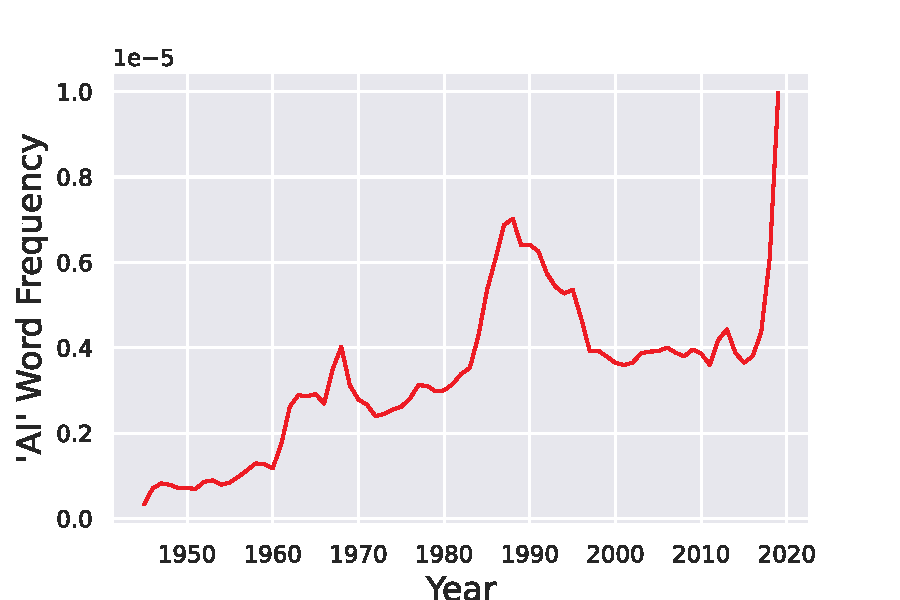
\includegraphics[width=0.7\textwidth]{images/introduction/ngramAI_good.pdf}
    \caption{Γραφική παράσταση της συχνότητας του όρου AI σε βιβλία γραμμένα στην αγγλική γλώσσα ανά έτος (από 1945 μέχρι και 2019). Είναι εμφανείς οι τρεις περίοδοι ακμής του κλάδου. Παράχθηκε από το \en{Google Ngram Viewer}. }
\end{figure}



\section{Κίνητρο}
\en{\blindtext[3]}
\section{Συνεισφορά Εργασίας}
\en{\blindtext[3]}
\section{Οργάνωση του Τόμου}

\en{\blindtext[3]} 
